\documentclass[conference]{IEEEtran}
\usepackage{cite}
\usepackage{url}
\usepackage[cmex10]{amsmath}
\usepackage{algorithm}
\usepackage{algpseudocode}
\usepackage{array}
\usepackage{mdwmath}
\usepackage{mdwtab}
\usepackage{eqparbox}
\usepackage{graphicx}
\usepackage {epsfig}
\usepackage{fixltx2e}
\usepackage{float}
\usepackage{graphicx}
\usepackage{caption}
\usepackage{subcaption}
\usepackage{threeparttable}

\begin{document}

\title{JavaScript Profiling and Optimization on V8}

\author{
\IEEEauthorblockN{Yilin Zhang}
\IEEEauthorblockA{zylime@gmail.com}
\and
\IEEEauthorblockN{C. Vic Hu}
\IEEEauthorblockA{vic@cvhu.org}
}

\maketitle

\begin{abstract}

In this course project, we want to focus on the trace profiling and optimizations in the V8 JavaScript Engine used in Google Chrome. By learning from their existing compiling infrastructure and optimization processes, we hope to extract the key essence out of the works done the V8 open source community, and to apply the optimization techniques covered in our class. Ultimately, we want to study what it takes to build a super fast JavaScript engine in the industry, and to see if we can come up with some feasible ideas to make some enhancements.

\end{abstract}

\section{Introduction}

Although JavaScript is traditionally translated into bytecode by an interpreter, more and more JavaScript Engines in modern browsers  are designed to compile directly into machine code. Our project will mainly focus on trace profiling\cite{Trace} in V8, and making constructive adjustments according to the optimization techniques we have learned in class. We will use the SunSpider JavaScript benchmark and the V8 benchmark to measure and compare the existing infrastructures, and make a sound analysis of the results. Our overall goal is to understand the common optimization procedures performed by modern JavaScript Engines, as well as the possible performance enhancements with the knowledge we've acquired from EE382V. 

In this paper, we will cover our motivations for doing this project, background information and detailed compilation processes about the V8 engine, profiling results, and comparisons to show the effectiveness of the optimizations done in V8.


%As we know internet riches people's life with new and quick information. At the same time people spend more and more timing browsing various websites. How to make the webpages response faster and save people's time becomes important. Infrastructure of cables and servers definitely play an important role, but compilation optimization\cite{Trace} and arrange the HTML tree\cite{Popularity} make difference when the infrastructure is unchangable.
%
%In this work, we will tackle both compilation optimization and arrangement of the HTML tree to accelerate the web response. We use TraceMonkey to help build the trace information and several optimization techniques are applied based on the trace structure. We analyze the web site popularity from the HTTP log file and then revise the HTTP tree based on the popularity.

\section{Motivation}
JavaScript has been widely used in web-based applications to increase richer interactions and visualizations \cite{mcduffie} since it was first supported by Netscape 2 beta back in 1995 \cite{jshistory}. In over fiften years, it has evolved into a variety of frameworks and libraries to enable a more interactive and dynamic web browsing experience \cite{ajax}, or even to build high-performance network programs \cite{node}. Besides its applications in web-based softwares, JavaScript has also gained its popularity from applications such as Adobe Flash, Dashboard widgets in Mac OSX, browser extensions, and web bookmarklets. Apart from its essential role in client-side interactions, JavaScript also became one of the mainstream server-side solutions in recent years\cite{node}. 

As the popularity of web-based applications and services increases, browser performance has become one of the major competitions in the industry. Since JavaScript is what makes modern web pages dynamic and interactive, how to optimize its compilation/interpretation is the key component to building fast and robust modern browsers. We compared modern web browsers on two JavaScript benchmarks, including Chrome Canary, Chrome, Firefox, Safari, and Opera. In Fig.\ref{figure:v8_benchmark}, it was clear that both Chrome Canary (the latest beta release) and Chrome significantly outperformed any other competitors among all the test cases in the V8 benchmark suites. In Fig.\ref{figure:spider_benchmark}, although it became less obvious that Chrome was superior than its peers in the SunSpider benchmark, we can still see the dominance of V8 in general. V8 benchmark suite was provided by the same community who developed the V8 engine, which was composed of some simulation benchmarks translated from other languages like BCPL, Smalltalk, and Scheme, as well as common operations and manipulation performance, while SunSpider mainly focused on utility performance such as text manipulation, encryption/decryption, data structure access, and common operations.



\begin{figure}[H]
	\begin{subfigure}[H]{0.5\textwidth}
		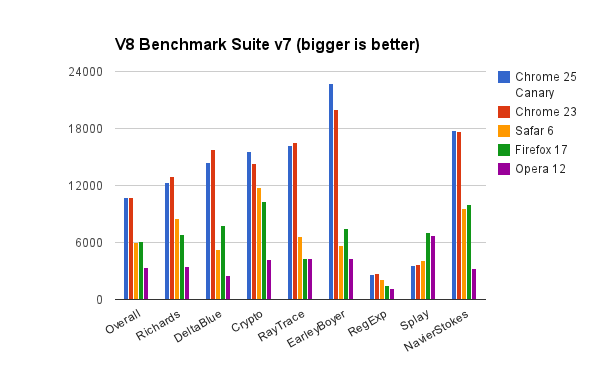
\includegraphics[width=\textwidth]{figs/v8_benchmark.png}
		 \caption{V8 Benchmark suite v7}
		 \label{figure:v8_benchmark}
	 \end{subfigure}
	\begin{subfigure}[H]{0.5\textwidth}
		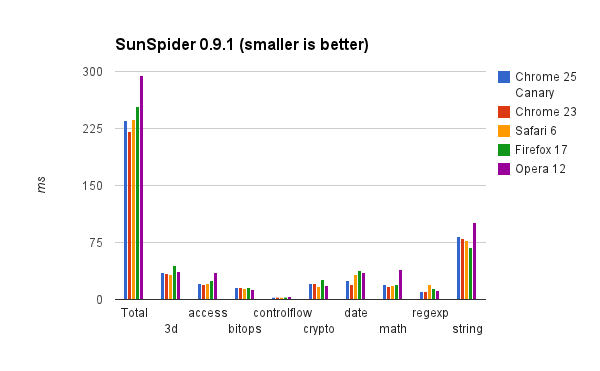
\includegraphics[width=\textwidth]{figs/sunspider_benchmark.png}
		\caption{SunSpider Benchmark v0.9.1}
		\label{figure:spider_benchmark}
	\end{subfigure}
	\caption{ Testing results on 2 common JavaScript Benchmarks}
\end{figure}

Although it has been pointed out that  the testing results from these popular JavaScript benchmarks don't necessarily indicate the true performance of real-world web applications \cite{jsmeter1}, the fact that Chrome dominated these competitions should somewhat reflect its success in designing a fast and efficient JavaScript engine. 

\section{Background}
In this section, we will talk about the high-level design and implementation of the most recent V8 JavaScript Engine (v3.15.10), with specific examples to explain the key concepts and principals that make V8 outstanding.

V8 is an open source project started in late 2006 by Google, which ships with their flagship Chrome web browser. Written in C++, V8 can run both as standalone and embedded applications. Its name came from the common automobile engine, and resembled the characteristics of being fast and efficient at the same time\cite{hc}.

\subsection{Key design concepts of V8}

\subsubsection{Fast property access}
As a dynamic programming language, object properties in JavaScript are dynamically modified in runtime, meaning that we can't just have a static memory location offset to access instance variables in programming languages like Java. In most JavaScript engines, property accesses are commonly implemented using a dynamic dictionary lookup to find the memory address, which is typically much slower and less efficient. 

The concept of hidden classes is to dynamically create and change the hidden class of an object whenever a new property is added. Let's look at a straightforward location class to see how it works:\\

\begin{verbatim}
function Location(lng, lat){
    this.lng = lng;
    this.lat = lat;
}
\end{verbatim}
\-\\

\begin{itemize}
\item Initialize a hidden class $C_0$ for Location objects with no properties to point to\\
\item When \texttt{lng} property is added, move the class pointer to a newly created hidden class $C_1$, which contains the offset of the \texttt{lng} property storage location. Update $C_0$ to redirect objects with property \texttt{lng} to $C_1$\\
\item When \texttt{lat} property is added, move the class pointer to a newly created hidden class $C_2$, which contains the offset of the \texttt{lat} property storage location. Update $C_1$ to redirect objects with property \texttt{lat} to $C_2$\\
\end{itemize}

Using this approach, most JavaScript programs share a large portion of hidden class structures during the runtime. The advantages of using hidden classes include dictionary lookup avoidance, which speeds up the time required for property accesses, and the opportunity of leveraging optimization with inline caching, which is a classic optimization technique to effectively eliminate the overhead in dynamic typing \cite{ic}.\\

\subsubsection{Dynamic machine code}
Unlike conventional interpreter for the most dynamic programming languages, V8 compiles JavaScript directly into machine code upon execution, without any intermediate byte codes. When property accessing code is initially executed, V8 fetches the current hidden class of the corresponding object and inserts the inline caching patches along with other machine instructions. 

Since V8 automatically predicts same hidden class used by all objects accessed in the same location, there might be incorrectly-patched inline caches with mismatched hidden classes, in which case V8 will handle the cache misses and redirect the object pointer to the correct hidden class. V8 also has a JavaScript regular expression engine, which was built from scratch to be automata-based and to produce machine code for regular expressions. 

Both the hidden classes techniques and the machine code generation provide benefits to speed and efficiency when many objects in the code share the same types and frequencies of property accesses, which can effectively improve the JavaScript runtime performance in most programs.\\


\subsubsection{Efficient garbage collection}


\subsection{V8 compilation process}

\subsubsection{Base compiler}

\subsubsection{Runtime profiler}

\subsubsection{Optimizing compiler}

\subsubsection{Deoptimization support}

%%%%%%Prime Algorithm starts here%%%%%%%%%%%%%%%%%%%%%%%%%%%%%%%%%%%%%%%%%%%%%%%%%%%%%%%%%%%%%%%%%%%%
\begin{algorithm}[hbt!]
	\caption{\scriptsize{\emph{Calculate the $25000$th Prime Number}}}
	 \label{algorithm:prime}
	 \begin{algorithmic}[1]
%		 \begin{scriptsize}			 
%\If {$i\geq maxval$}
%    \State $i\gets 0$
%\Else
%    \If {$i+k\leq maxval$}
%        \State $i\gets i+k$
%    \EndIf
%\EndIf
			\Require
			 \Ensure {The $25000$th Prime Number P}
			 \State {Prime list PL = \{\}} 
			 \For {P = 1 to infinity}
			    \State {Flag = true}
			    \For{index = 1 to PL.size()}
			 	\If {P.mod(PL[i]) == 0}
			            \State {Flag = false}
			            \State {Continue}
			        \EndIf
			    \EndFor
			    \If {Flag == true}
			        \State {PL.push\_back(P)}
			        \If {PL.size() == 25000}
			            \Return {PL.back()}
			        \EndIf
			     \EndIf
			  \EndFor
%		\end{scriptsize}
	\end{algorithmic}
\end{algorithm}

%%%%%%%%%%%%%%%%%%%%%%%%%%%%%%%%%%%%%%%%%%%%%%%%%%%%%%%%%%%%%%%%%%%%%%%%%%%%%%%%%%%%%%%%%%%%%%%%%%
\section{Approach}
JavaScript is slow mainly due to JavaScript programs are untyped, and then compiled and run on the fly. Dynamic compilation is a great complement to static one. But completely replacing the optimized-to-death static compilation with JIT will lose the performance. 
\begin{figure}[h]	
         \centering
         \begin{subfigure}[H]{0.66\textwidth}%in [] it for caption
            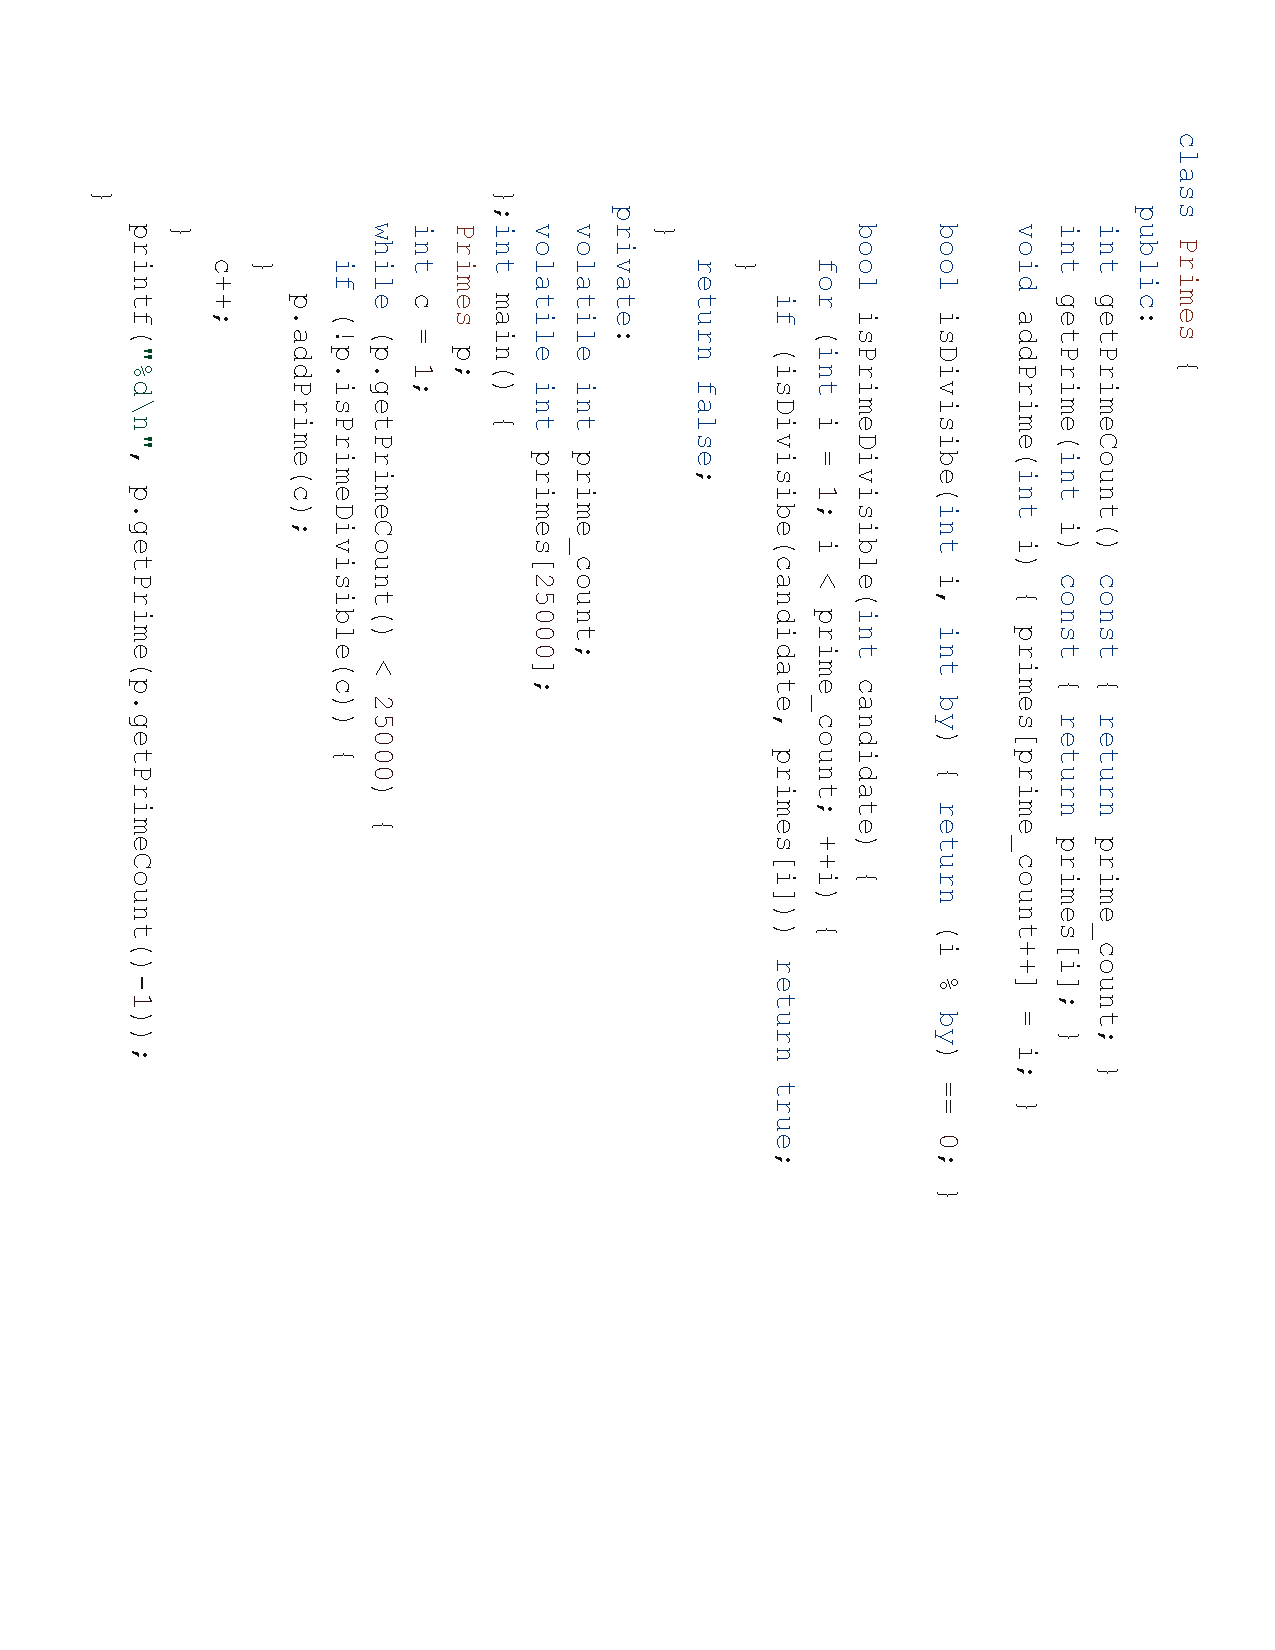
\includegraphics[width=\textwidth]{figs/prime_cplusplus}
            \caption{ C++ }
            \label{figure:prime_cplusplus}            
        \end{subfigure}
        
        \begin{subfigure}[H]{0.66\textwidth}
            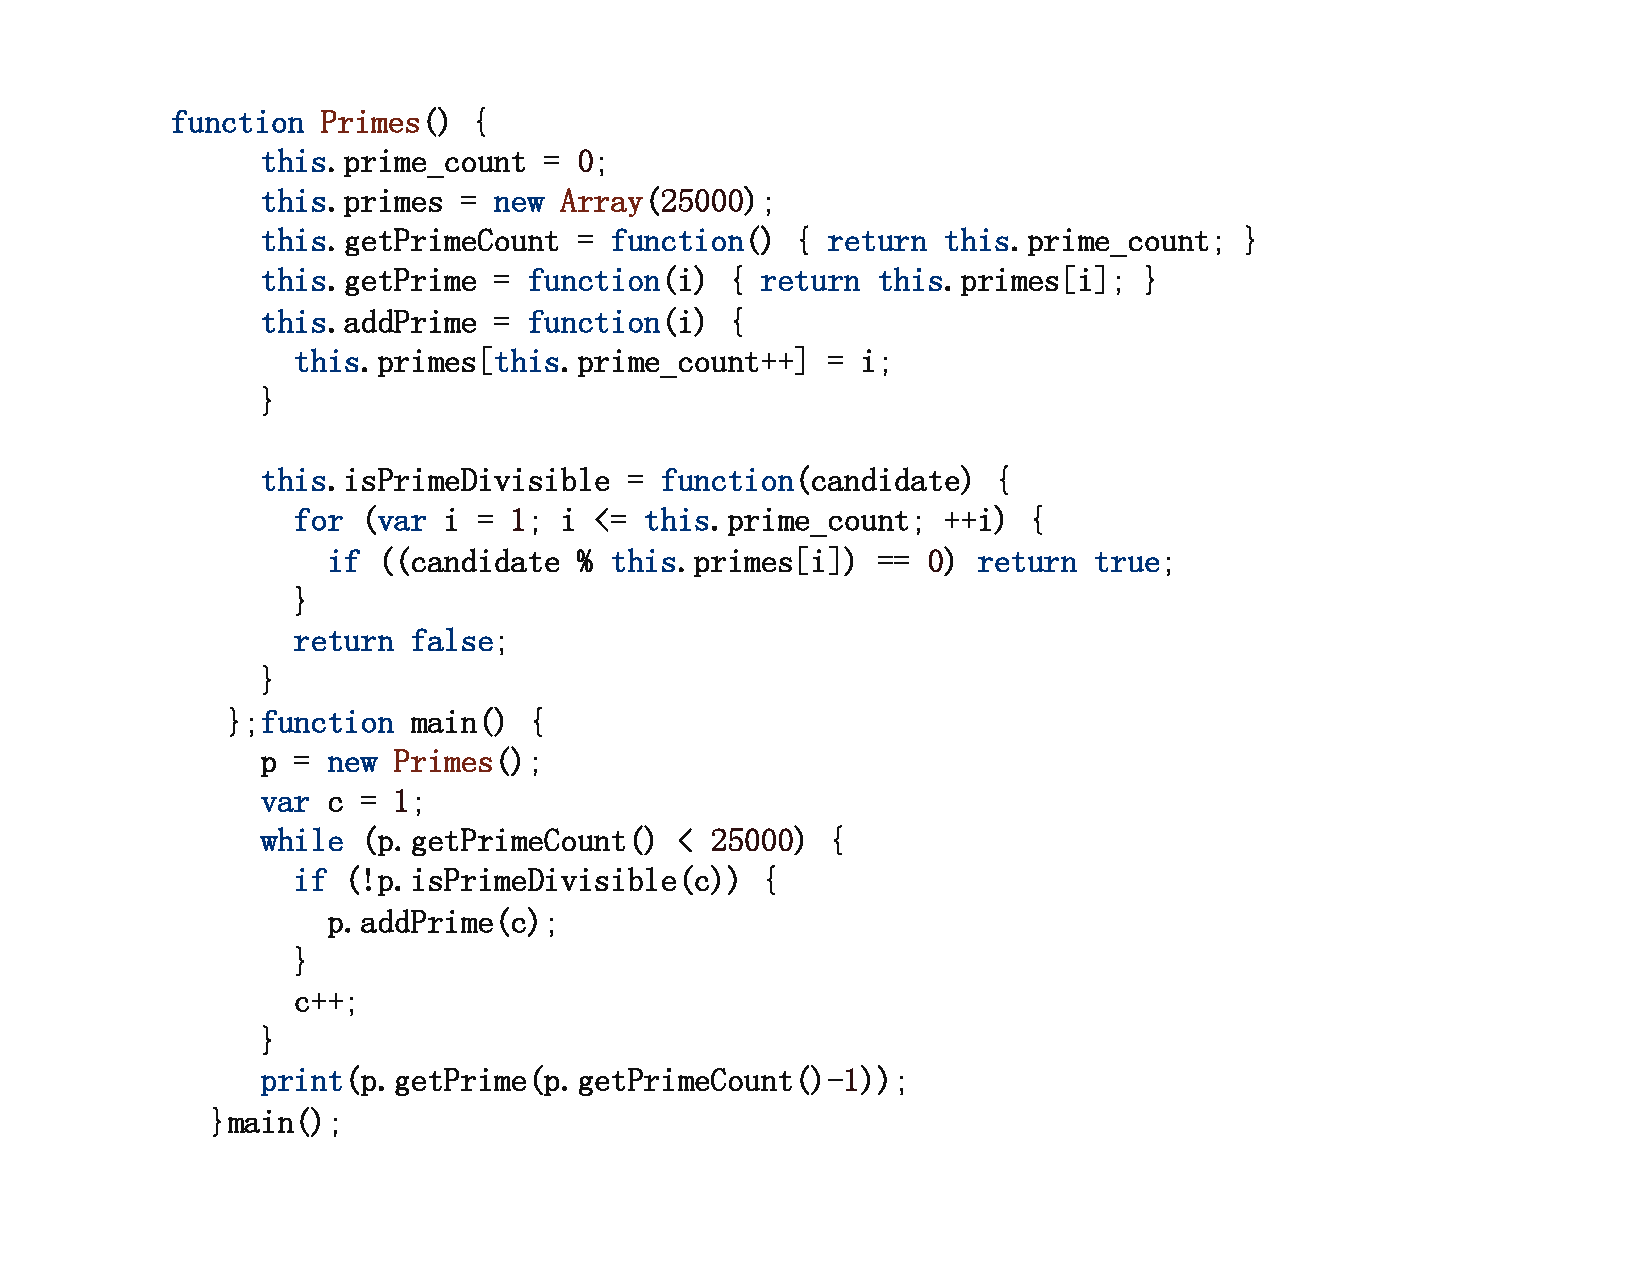
\includegraphics[width=\textwidth]{figs/prime_JavaScript}
            \caption{JavaScript}
            \label{figure:prime_JavaScript}
        \end{subfigure}
    	\caption{the code of calculating the $25000$th prime number}
    	\label{figure:prime}
\end{figure}
JavaScript is slower compared with other programming languages, such as C++. Before applying the optimization to the compilation of JavaScript code, we used one example to demonstrate how slow JavaScript was compared with C++. 
%\begin{figure}[hbt!]
%    \centering
%        \subfigure[]{
%            \label{figure:prime_cplusplus}
%            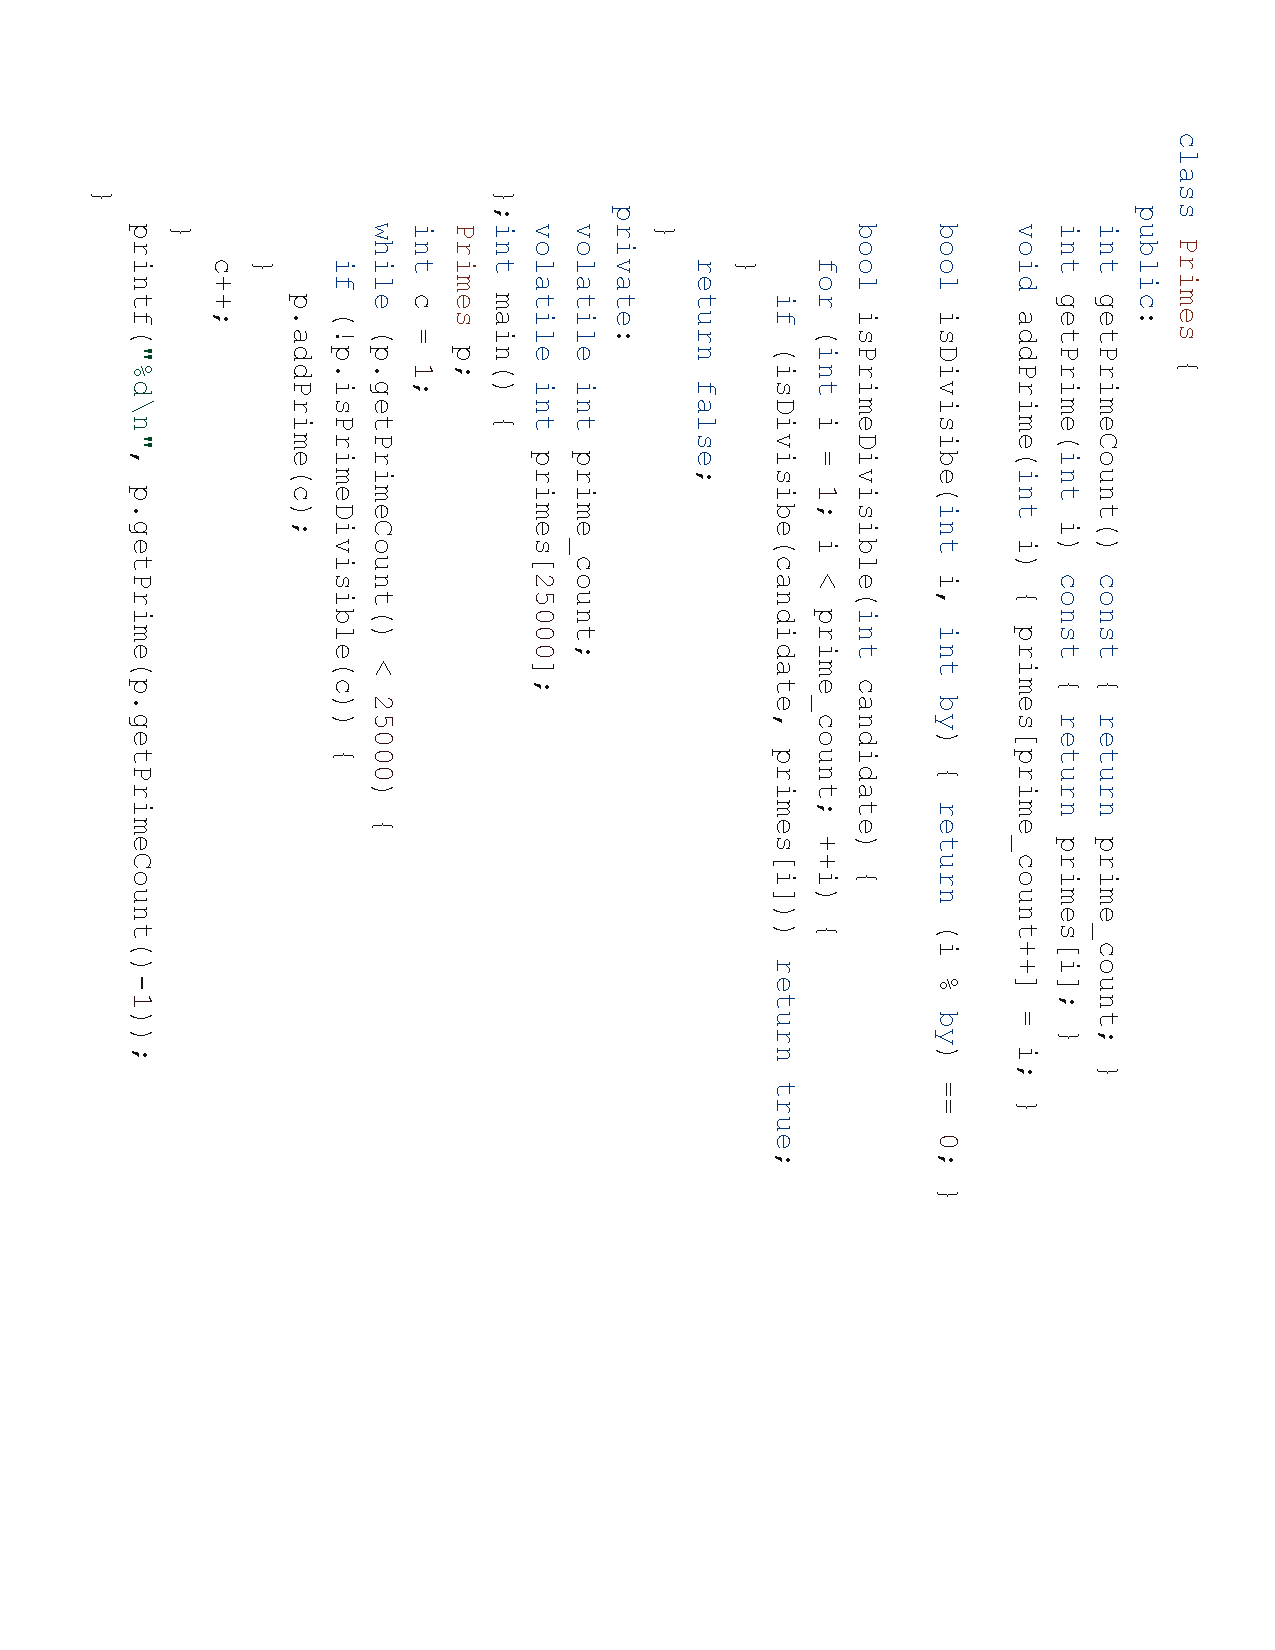
\includegraphics[width=0.64\textwidth]{figs/prime_cplusplus}
%        }
%        \subfigure[]{
%           \label{figure:prime_JavaScript}
%           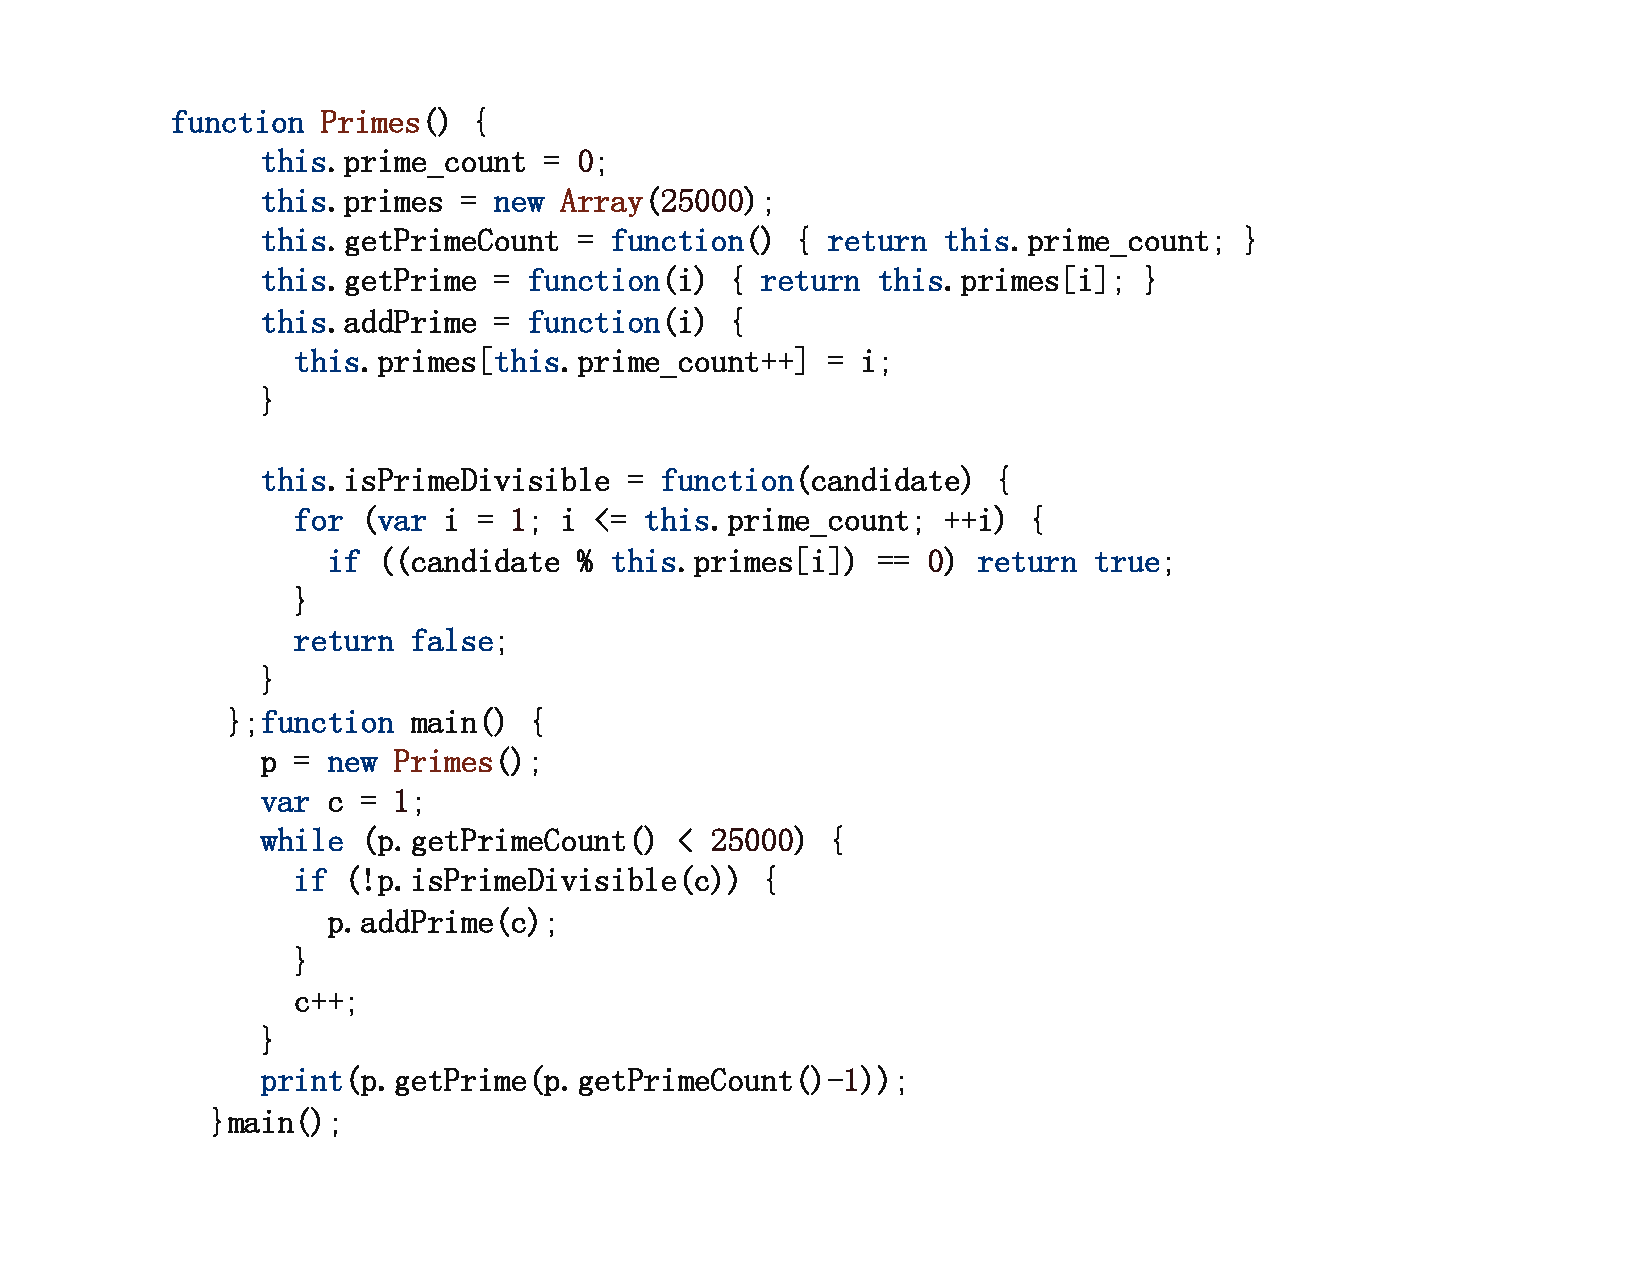
\includegraphics[width=0.64\textwidth]{figs/prime_JavaScript}
%        }
%    \caption{(a) was the C++ code of calculating the $25000$th prime number (b) was the JavaScript code for $25000$th prime number.}
%	\label{figure:prime}
% \end{figure}
\begin{figure}[h]
    \centering
    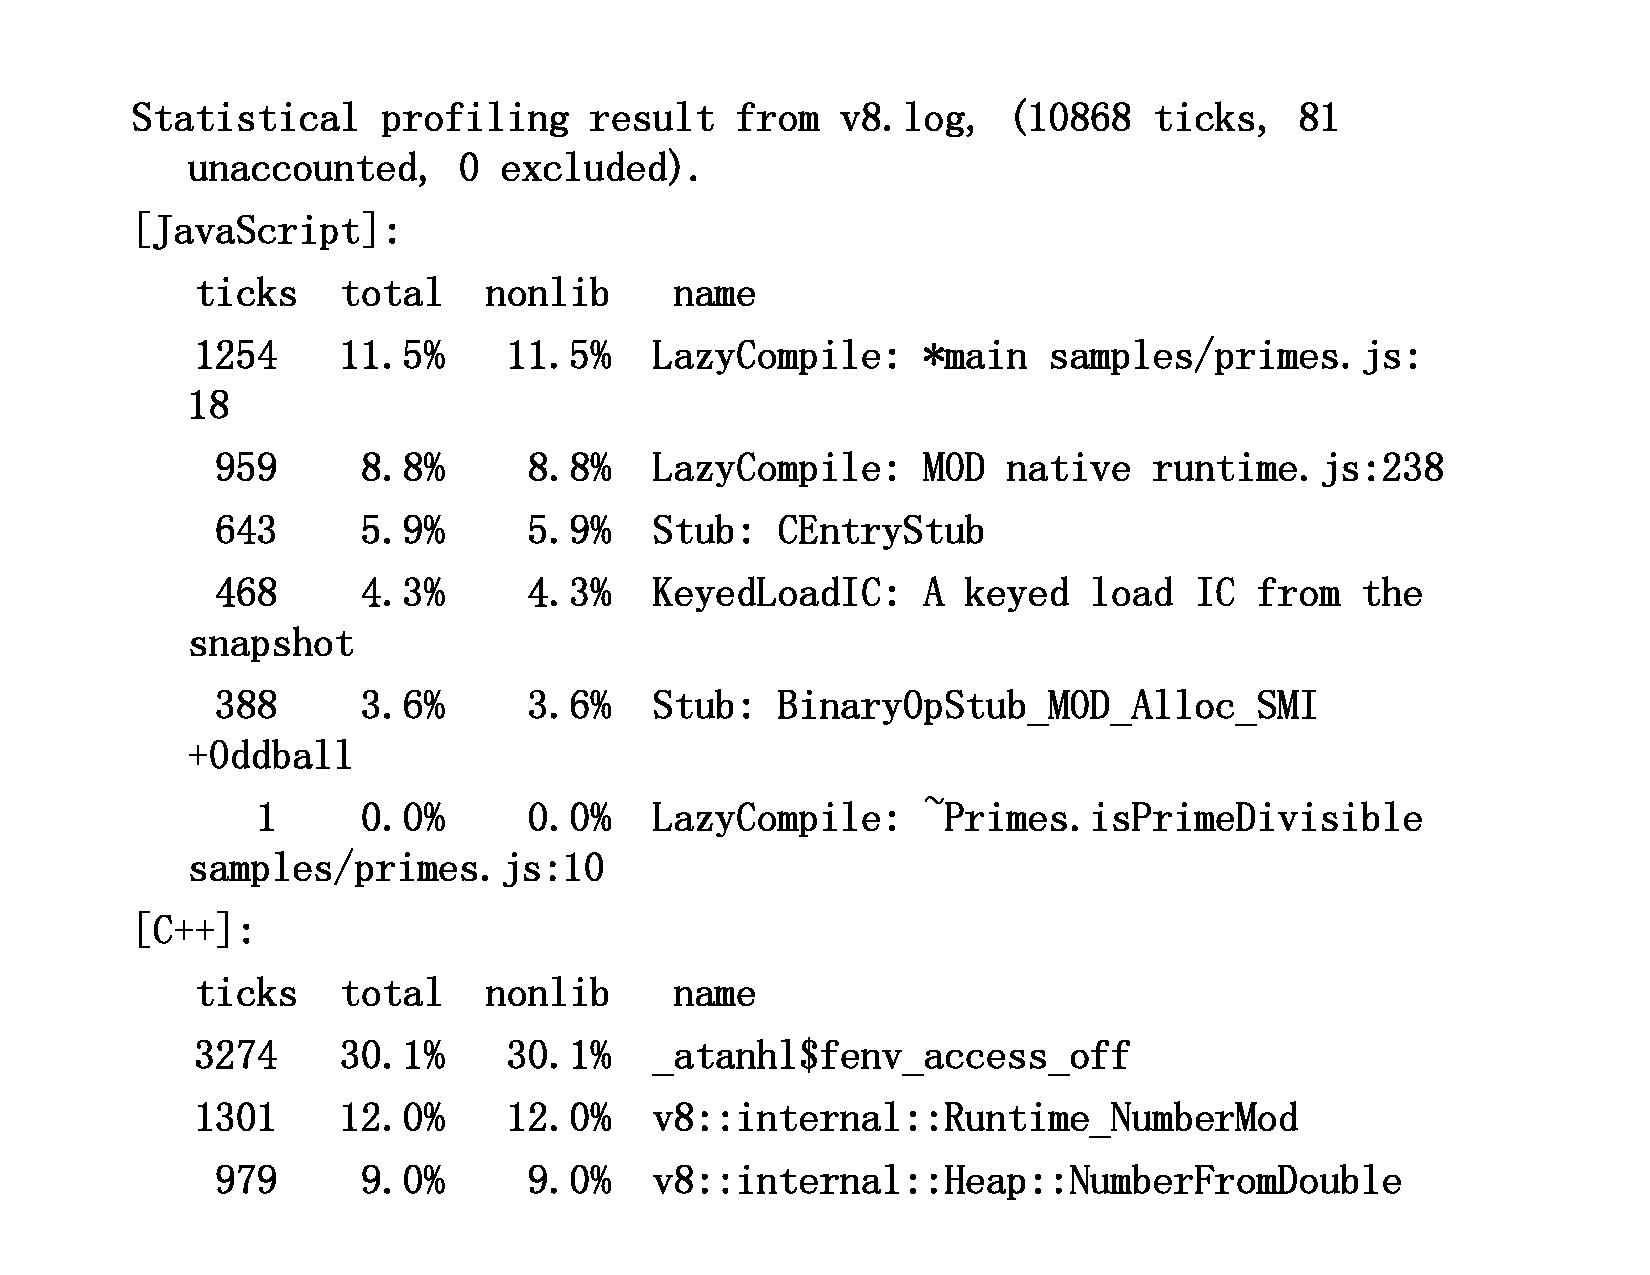
\includegraphics[width=0.54\textwidth]{figs/prime_profiling}
    \caption{ }
    \label{figure:prime_profiling}
 \end{figure}

The example here was to calculate the $25000$th prime number\cite{googleIO}. The overall algorithm of calculating the $25000$th prime number was illustrated in Algorithm\ref{algorithm:prime}.
The C++ code implementing the algorithm was in the Fig.\ref{figure:prime_cplusplus} while the JavaScript version was in the Fig.\ref{figure:prime_JavaScript}.
Running these two different versions of code on the same machine showed that the runtime of C++ code was 5x faster than the JavaScript code. To find the reason of poor performance of the JavaScript code, we performed a profiling on the JavaScript code to determine the runtime of each function.
First, We executed the command in \eqref{eq:1} to get the log file with profiling information. 
\begin{align}
  \scriptsize & ./out/ia32.release/d8 samples/primes.js --prof\label{eq:1}
\end{align}
Second, \eqref{eq:2} was applied to get the extract the runtime information of each function from the log file. 
\begin{align}
./tools/mac-tick-processor v8.log\label{eq:2}
\end{align}
The output of \eqref{eq:2} provides us the runtime of each function in the JavaScript code, as in Fig.\ref{figure:prime_profiling}.


Beyond our expectation, the most runtime was not spent on the main function. The main function only consumed less than 12\% of the total runtime while about 30\% of the total runtime was spent on the function env\_access\_off. With this hint, we noticed that the access of the last element, this.prime[this.prime\_count], was out of the range of identified prime numbers. 
Though with this incorrect access, JavaScript could still give the correct $25000$th prime number - 287107, the runtime increased drametically.

By correcting the access range in the isPrimeDivisible function, the new run time was only about 1.17 times of the C++ code. This improvement illustrated that JavaScript was slower tan C++, but was not much slower. 
The profiling with the out-of-bounds fixed was in Fig.\ref{figure:prime_profiling_2}. From the new profiling, we could observe that more than 99\% was spent on the main function.
\begin{figure}[H]
    \centering
    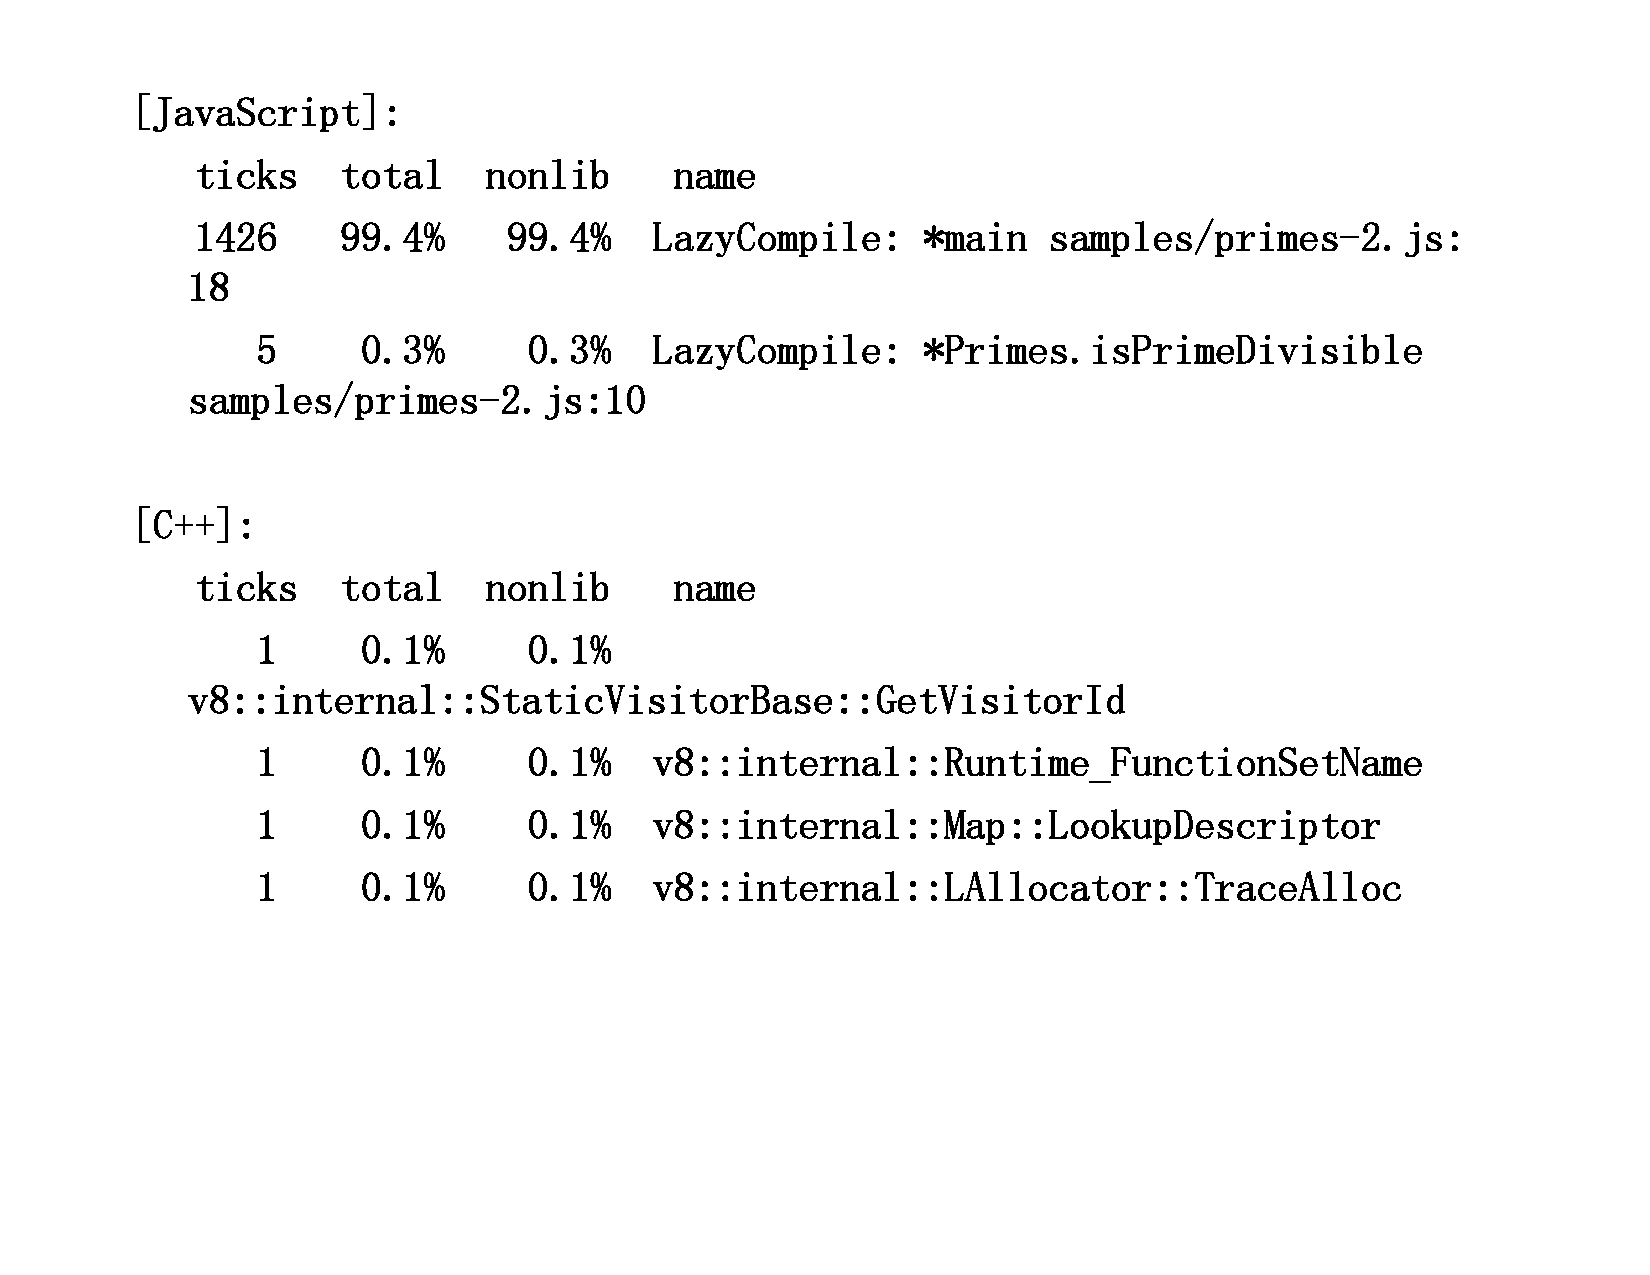
\includegraphics[width=0.54\textwidth]{figs/prime_profiling_2}
    \caption{ }
    \label{figure:prime_profiling_2}
\end{figure}


\section{Results}
The experiments are conducted on an Intel Core i7 2.3GHz Mac OS X  with 8GB memory.
In Table~\ref{table:result1}, we compare the runtime of the C++ code with the JavaScript version in Fig.\ref{figure:prime}.
%%%%%%%%%%%%%%%%%%%%%%%%%%%%%%%%%%%%%%%%%%%%%%%%%%%%%%%%%%%%%%%%%%%%%%%%%
%\vspace{-0.2in}
%\begin{table*} [hbt!]
\begin{table*} [hbt!]
%\vspace{-0.1in}
\centering
\caption{Comparisons between C++, JavaScript and Improved JavaScript}
\label{table:result1}
\begin{threeparttable}
\begin{scriptsize}
\begin{tabular}{|c|c|c|c|c|c|c|c|c|c|c|c|}
\hline
Benchmarks & \multicolumn{3}{|c}{C++} & \multicolumn{4}{|c}{JavaScript} & \multicolumn{4}{|c|}{Improved JavaScript}\\
\cline{2-12}
           & real (s)& user (s) & sys (s)& real (s)& user (s) & sys (s)& \% of main & real (s)& user (s) & sys (s)& \% of main\\
\hline
\end{tabular}
\end{scriptsize}
%\begin{tablenotes}
%\begin{scriptsize}
%\item [a] Each WDM trunk has up to 32 available channels at initial placement. Unassigned trunks will be turned off after routing.
%\item [b] Unassigned WDM channels will be turned off (no laser input from off-chip) in the global routing stage.
%\item [c] Total power consumption is normalized to the power consumed on CK1 by \emph{GLOW}.
%\end{scriptsize}
%\end{tablenotes}
\end{threeparttable}
\vspace{-0.2in}
\end{table*}
%%%%%%%%%%%%%%%%%%%%%%%%%%%%%%%%%%%%%%%

\section{Conclusion}

\section{Acknoledgment}
We are very grateful to Dr. Vijay Reddi for the discussions and advices to the scope and direction of this paper.

%\begin{figure}[hbt!]	
%         \centering
%         \begin{subfigure}[b]{0.55\textwidth}%in [] it for caption
%            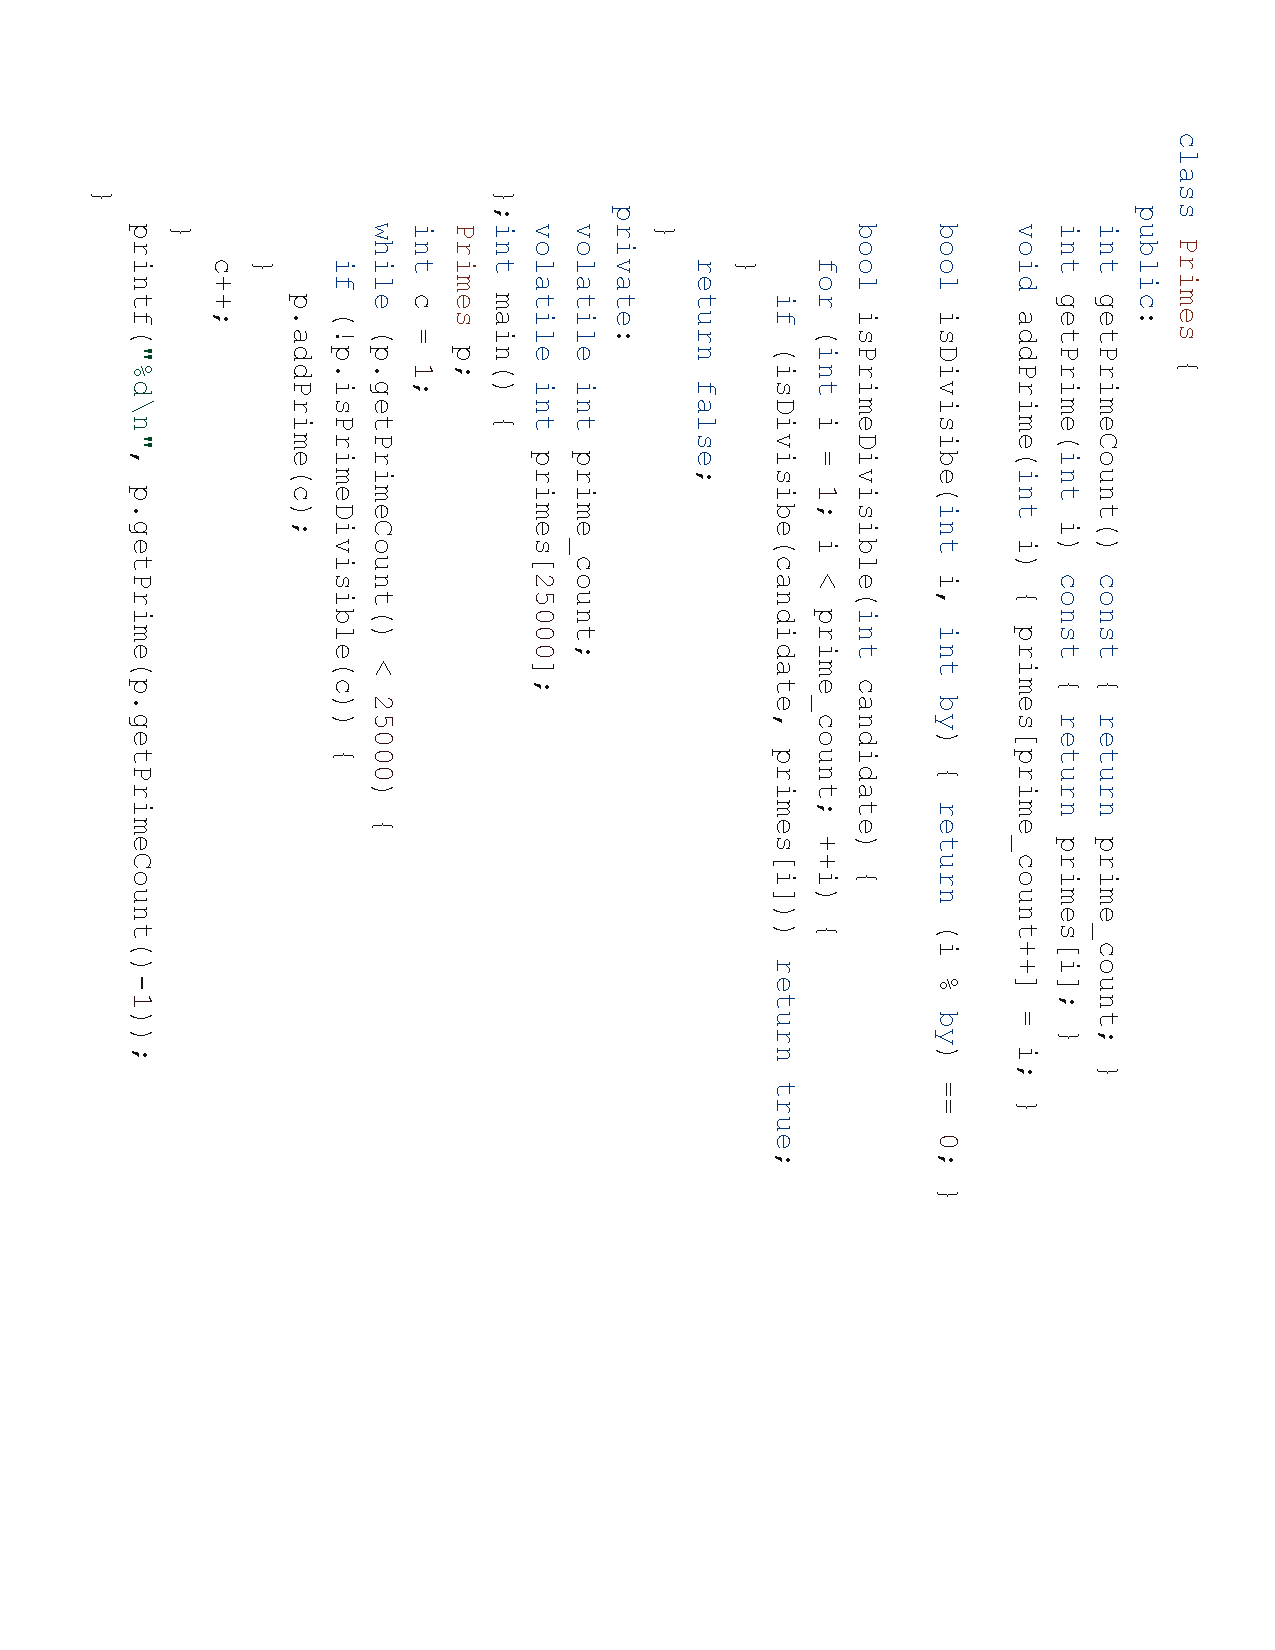
\includegraphics[width=\textwidth, angle=90]{figs/prime_cplusplus}
%            \caption{ C++ }
%            \label{figure:prime_cplusplus}            
%        \end{subfigure}
%        
%        \begin{subfigure}[b]{0.55\textwidth}
%            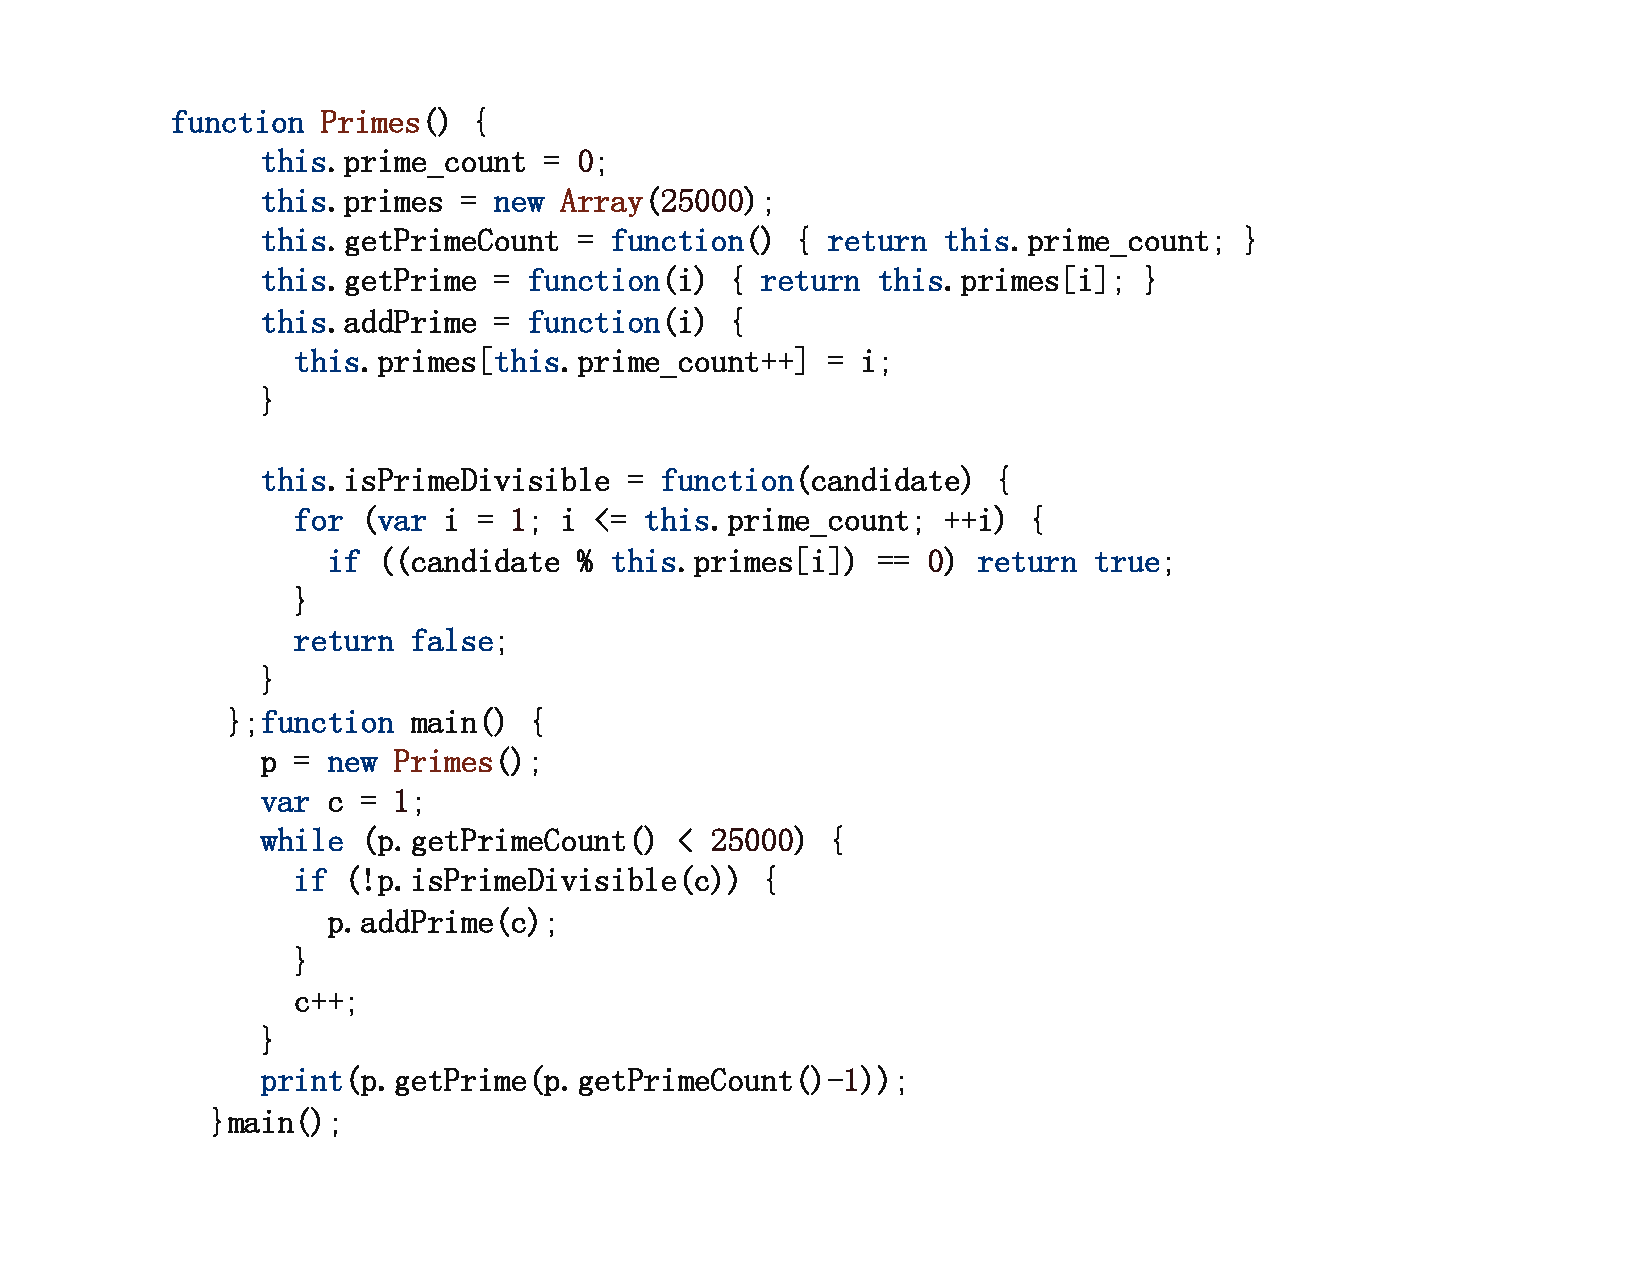
\includegraphics[width=\textwidth, angle=90]{figs/prime_JavaScript}
%            \caption{JavaScript}
%            \label{figure:prime_JavaScript}
%        \end{subfigure}
%    	\caption{the code of calculating the $25000$th prime number}
%    	\label{figure:prime}
%\end{figure}


%
%
%
%\section{Approach}
%
%
%

%
%\section{Results}
%
%\subsection{Experimental Framework}
%
%
%
%\subsection{Data}
%
%
%
%
%
%\begin{table}[h]
%% increase table row spacing, adjust to taste
%\renewcommand{\arraystretch}{1.3}
%\caption{There is no period in a table caption}
%\label{table_example}
%\centering
%% Some packages, such as MDW tools, offer better commands for making tables
%% than the plain LaTeX2e tabular which is used here.
%\begin{tabular}{|c||c|}
%\hline
%One & Two\\
%\hline
%Three & Four\\
%\hline
%\end{tabular}
%\end{table}
%\renewcommand{\arraystretch}{1}
%
%\section{Related Work}
%
%
%
%\section{Conclusion}
%
%
%
%\section*{Acknowledgment}


\begin{thebibliography}{1}

\bibitem{jshistory}
Eich, Brendan. "JavaScript at ten years." ACM SIGPLAN Notices. Vol. 40. No. 9. ACM, 2005.
\bibitem{mcduffie}
McDuffie, Tina. JavaScript Concepts \& Techniques: Programming Interactive Web Sites. Franklin Beedle \& Associates, 2003.
\bibitem{ajax}
Serrano, Nicol�s, and Juan Pablo Aroztegi. "Ajax frameworks in interactive web apps." Software, IEEE 24.5 (2007): 12-14.
\bibitem{node}
Tilkov, Stefan, and Steve Vinoski. "Node. js: Using JavaScript to build high-performance network programs." Internet Computing, IEEE 14.6 (2010): 80-83.

\bibitem{jsmeter1}
Ratanaworabhan, Paruj, Benjamin Livshits, and Benjamin G. Zorn. "JSMeter: Comparing the behavior of JavaScript benchmarks with real web applications." Proceedings of the 2010 USENIX conference on Web application development. USENIX Association, 2010.

\bibitem{hc}
Gray, James. "Google Chrome: the making of a cross-platform browser." Linux Journal 2009.185 (2009): 1.


\bibitem{ic}
Brunthaler, Stefan. "Efficient inline caching without dynamic translation." Proceedings of the 2010 ACM Symposium on Applied Computing. ACM, 2010.
%\bibitem{IEEEhowto:kopka}
%H.~Kopka and P.~W. Daly, \emph{A Guide to \LaTeX}, 3rd~ed.\hskip 1em plus
%  0.5em minus 0.4em\relax Harlow, England: Addison-Wesley, 1999.
\bibitem{Trace}
Jungwoo Ha and Mohammad R. Haghighat and Shengnan Cong, A concurrent trace-based just-in-time compiler for javascript, Tech Report, 2009
\bibitem{Popularity}
John Garofalakis and Panagiotis Kappos and Dimitris Mourloukos, Web site optimization using page popularity, Internet Computing, 1999
\bibitem{node}
"Why Everyone Is Talking About Node." Jolie O'Dell. Mashable, Inc., Web. 10 Mar. 2011.
\bibitem{googleIO}
"Breaking the JavaScript Speed Limit with V8", Google I/O, 2012

\end{thebibliography}




% that's all folks
\end{document}
